%  Adaptive 2D Coarsening for the RDME — conference talk
%  Aditya Dendukuri

\documentclass[10pt,aspectratio=169]{beamer}

\usetheme{Boadilla}
\usecolortheme{seahorse}
\setbeamertemplate{navigation symbols}{}
\setbeamerfont{frametitle}{size=\normalsize,series=\bfseries}
\setbeamerfont{title}{size=\large,series=\bfseries}
\setbeamertemplate{bibliography item}[text]

\usepackage{amsmath,amssymb,bm,mathtools}
\usepackage{tikz}
\usepackage{ifthen}
\usetikzlibrary{arrows.meta,positioning,patterns,decorations.pathreplacing,calc,fit}
\usepackage{graphicx}
\usepackage{booktabs}
\usepackage{xcolor}

\graphicspath{{figures/}}

\newcommand{\Mult}{\operatorname{Mult}}
\newcommand{\citeref}[1]{{\scriptsize\textcolor{gray}{[#1]}}}

\definecolor{settledblue}{RGB}{31,119,180}
\definecolor{activeorange}{RGB}{255,127,14}
\definecolor{emptygray}{RGB}{180,180,180}
\definecolor{myblue}{RGB}{31,119,180}
\definecolor{mygray}{RGB}{80,80,80}
\definecolor{slowred}{RGB}{214,39,40}

\title[Adaptive 2D Coarsening for RDME FSP]{%
  Adaptive Spatial Coarsening\\
  for the Reaction-Diffusion Master Equation}
\author{Aditya Dendukuri}
\institute[UCSB]{University of California, Santa Barbara}
\date{}

\begin{document}

\begin{frame}\titlepage\end{frame}

% ================================================================
%  1. Setting: RDME and the dimensionality problem
% ================================================================
\begin{frame}{Stochastic reaction-diffusion: the RDME}

\begin{columns}[T]
\begin{column}{0.52\textwidth}
  Molecules live on a spatial grid of $K$ voxels.\\[0.5em]
  State: $\mathbf{n} = (n_1,\ldots,n_K)\in\mathbb{Z}_{\ge 0}^K$\\
  (molecule count per voxel)\\[0.8em]

  \textbf{Two types of events:}
  \begin{enumerate}
    \item \textbf{Reactions} — local, within each voxel\\
          $\varnothing \xrightarrow{\lambda} X,\quad X \xrightarrow{\mu n_k} \varnothing$
    \item \textbf{Diffusion} — molecules hop to adjacent voxels\\
          $X_k \xrightarrow{D/h^2\cdot n_k} X_{k\pm 1}$
  \end{enumerate}

  \bigskip
  The probability $p(\mathbf{n},t)$ satisfies the \textbf{RDME}:
  \[
    \dot{p} = A\,p,
  \]
  $A$ is a sparse matrix encoding every hop and reaction event.
\end{column}
\begin{column}{0.45\textwidth}
  \centering
  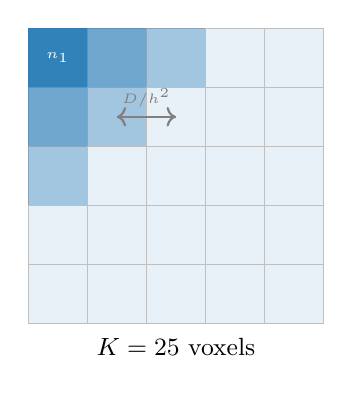
\begin{tikzpicture}[scale=0.75]
    % 5x5 grid with gradient coloring (manual)
    \foreach \i in {0,...,4} \foreach \j in {0,...,4} {
      \draw[gray!50,fill=myblue!10] (\j,4-\i) rectangle (\j+1,5-\i);
    }
    % Brighter corner
    \fill[myblue,opacity=0.9] (0,4) rectangle (1,5);
    \fill[myblue,opacity=0.6] (1,4) rectangle (2,5);
    \fill[myblue,opacity=0.6] (0,3) rectangle (1,4);
    \fill[myblue,opacity=0.35] (2,4) rectangle (3,5);
    \fill[myblue,opacity=0.35] (1,3) rectangle (2,4);
    \fill[myblue,opacity=0.35] (0,2) rectangle (1,3);
    % arrows for diffusion
    \draw[->,thick,gray] (1.5,3.5) -- (2.5,3.5) node[midway,above,font=\tiny] {$D/h^2$};
    \draw[->,thick,gray] (2.5,3.5) -- (1.5,3.5);
    \node[font=\tiny,white] at (0.5,4.5) {$n_1$};
    \node[font=\small] at (2.5,-0.4) {$K = 25$ voxels};
  \end{tikzpicture}

  \bigskip
  \begin{alertblock}{The problem}
    State space $\sim n_{\max}^K$.\\
    $K=400$ voxels, $n_{\max}=10$: $10^{400}$ states.
  \end{alertblock}
\end{column}
\end{columns}
\end{frame}

% ================================================================
%  2. FSP: solving the RDME exactly
% ================================================================
\begin{frame}{Finite State Projection: exact distributions at finite cost}

\begin{columns}[T]
\begin{column}{0.55\textwidth}
  \textbf{FSP} \citeref{Munsky \& Khammash 2006}: truncate $A$ to a finite support
  $\mathcal{S}\subset\mathbb{Z}_{\ge 0}^K$ and solve
  \[
    \dot{p}_{\mathcal{S}} = A_{\mathcal{S}}\,p_{\mathcal{S}}.
  \]

  \medskip
  Adaptively grow $\mathcal{S}$ until the truncation error is below tolerance.\\[0.8em]

  \textbf{Cost:} $|\mathcal{S}|$ equations to solve.\\[0.4em]
  $|\mathcal{S}|$ grows exponentially in $K$: intractable for large grids.

  \bigskip
  \textbf{Key question:}\\[0.3em]
  Can we reduce the effective dimensionality of the problem
  by exploiting spatial structure?
\end{column}
\begin{column}{0.42\textwidth}
  \centering
  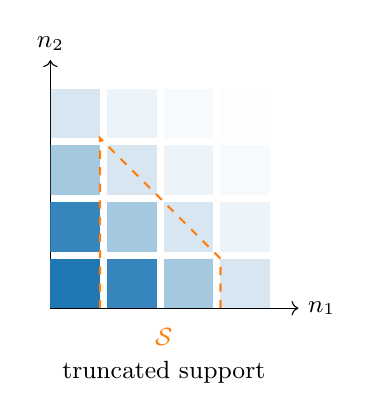
\begin{tikzpicture}[scale=0.9]
    % state space grid for K=2
    \draw[->] (0,0) -- (3.5,0) node[right,font=\small] {$n_1$};
    \draw[->] (0,0) -- (0,3.5) node[above,font=\small] {$n_2$};
    \foreach \i in {0,...,3} \foreach \j in {0,...,3} {
      \pgfmathsetmacro\p{exp(-(\i+\j)*0.8)*2}
      \fill[myblue,opacity=\p] (\i*0.8,\j*0.8) rectangle (\i*0.8+0.7,\j*0.8+0.7);
    }
    \draw[dashed,thick,activeorange] (0.7,0) -- (0.7,2.4) -- (2.4,0.7) -- (2.4,0);
    \node[font=\small,activeorange] at (1.6,-0.4) {$\mathcal{S}$};
    \node[font=\small] at (1.6,-0.9) {\small truncated support};
  \end{tikzpicture}

  \bigskip
  {\small FSP is exact for well-mixed (CME) systems.\\
  For $K$ voxels: $|\mathcal{S}| \sim n_{\max}^K$.}
\end{column}
\end{columns}
\end{frame}

% ================================================================
%  3. The key insight: homogeneity = CME
% ================================================================
\begin{frame}{When does the RDME reduce to the CME?}

\begin{columns}[T]
\begin{column}{0.55\textwidth}
  \textbf{Observation:} when all $K$ voxels hold the same
  distribution (spatial homogeneity), tracking each voxel
  separately is redundant.

  \bigskip
  If $p(\mathbf{n},t) = p_{\rm CME}(N,t)\cdot\Mult(N;\tfrac{1}{K},\ldots,\tfrac{1}{K})$\\[0.5em]
  then we only need to track the \emph{total count} $N = \sum_k n_k$.

  \bigskip
  \begin{block}{RDME $\to$ CME}
    Spatial homogeneity $\Leftrightarrow$ the $K$-dimensional RDME
    collapses to a 1-dimensional CME for the total count.\\[0.4em]
    State space: $n_{\max}^K \to n_{\max}$.
  \end{block}

  \medskip
  \textbf{When does this happen?}\\
  Fast diffusion, or steady state, or large $t$.
\end{column}
\begin{column}{0.42\textwidth}
  \centering
  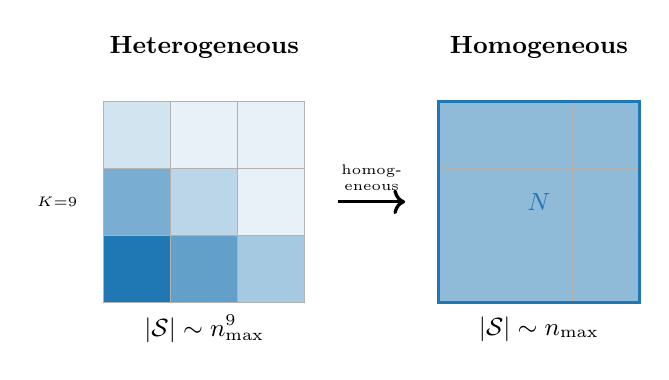
\begin{tikzpicture}[scale=0.85]
    % Heterogeneous
    \node[font=\small\bfseries] at (1.5,3.8) {Heterogeneous};
    \foreach \i in {0,...,2} \foreach \j in {0,...,2} {
      \pgfmathsetmacro\val{max(0.1, 1-0.4*\i-0.3*\j)}
      \fill[myblue,opacity=\val] (\j,\i) rectangle (\j+1,\i+1);
      \draw[gray!60] (\j,\i) rectangle (\j+1,\i+1);
    }
    \node[font=\tiny] at (-0.7,1.5) {$K{=}9$};
    \node[font=\small] at (1.5,-0.4) {$|\mathcal{S}| \sim n_{\max}^9$};

    % Arrow
    \draw[->,very thick] (3.5,1.5) -- (4.5,1.5)
      node[midway,above,font=\tiny,align=center]{homog-\\eneous};

    % Homogeneous
    \node[font=\small\bfseries] at (6.5,3.8) {Homogeneous};
    \fill[myblue,opacity=0.5] (5,0) rectangle (8,3);
    \draw[gray!60] (5,0) rectangle (8,3);
    \draw[gray!60] (6,0) -- (6,3); \draw[gray!60] (7,0) -- (7,3);
    \draw[gray!60] (5,1) -- (8,1); \draw[gray!60] (5,2) -- (8,2);
    \draw[very thick,settledblue] (5,0) rectangle (8,3);
    \node[font=\small,settledblue] at (6.5,1.5) {$N$};
    \node[font=\small] at (6.5,-0.4) {$|\mathcal{S}| \sim n_{\max}$};
  \end{tikzpicture}

  \medskip
  {\small The spatially uniform state is a\\ single merged super-voxel = CME.}
\end{column}
\end{columns}
\end{frame}

% ================================================================
%  4. The idea: merge low-activity voxels
% ================================================================
\begin{frame}{Adaptive coarsening: merge where activity is low}

\textbf{Principle:} voxels with \emph{low net diffusion activity}
can be merged without accuracy loss.

\bigskip
\begin{columns}[T]
\begin{column}{0.32\textwidth}
  \centering
  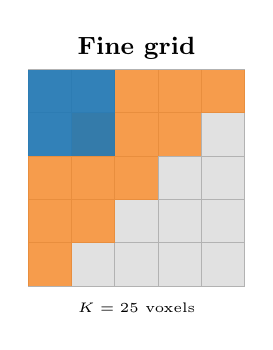
\begin{tikzpicture}[scale=0.55]
    % empty background
    \foreach \i in {0,...,4} \foreach \j in {0,...,4} {
      \fill[emptygray,opacity=0.4] (\j,4-\i) rectangle (\j+1,5-\i);
      \draw[gray!60] (\j,4-\i) rectangle (\j+1,5-\i);
    }
    % active: diagonal band
    \foreach \i/\j in {0/2,0/3,0/4,1/1,1/2,1/3,2/0,2/1,2/2,3/0,3/1,4/0} {
      \fill[activeorange,opacity=0.7] (\j,4-\i) rectangle (\j+1,5-\i);
    }
    % settled: top-left 2x2
    \foreach \i/\j in {0/0,0/1,1/0,1/1} {
      \fill[settledblue,opacity=0.9] (\j,4-\i) rectangle (\j+1,5-\i);
    }
    \node[font=\small\bfseries] at (2.5,5.5) {Fine grid};
    \node[font=\tiny] at (2.5,-0.5) {$K = 25$ voxels};
  \end{tikzpicture}
\end{column}
\begin{column}{0.10\textwidth}
  \centering
  \vspace{1.5cm}
  $\xrightarrow{\text{coarsen}}$
\end{column}
\begin{column}{0.32\textwidth}
  \centering
  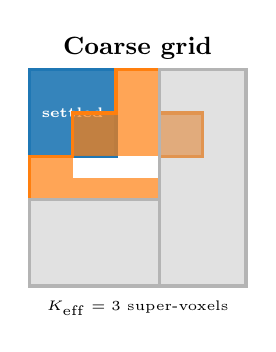
\begin{tikzpicture}[scale=0.55]
    % settled: top-left 2x2 block
    \fill[settledblue,opacity=0.9] (0,3) rectangle (2,5);
    \draw[settledblue,very thick] (0,3) rectangle (2,5);
    \node[white,font=\tiny\bfseries] at (1,4) {settled};

    % active front: staircase shape
    \fill[activeorange,opacity=0.7] (2,4) rectangle (3,5);
    \fill[activeorange,opacity=0.7] (1,3) rectangle (2,4);
    \fill[activeorange,opacity=0.7] (2,3) rectangle (4,4);
    \fill[activeorange,opacity=0.7] (0,2) rectangle (1,3);
    \fill[activeorange,opacity=0.7] (1,2) rectangle (3,2.5);
    \draw[activeorange,very thick]
      (0,2)--(0,3)--(1,3)--(1,4)--(2,4)--(2,5)--(3,5)--(3,4)--(4,4)--(4,3)--(3,3)--(3,2)--(0,2);

    % empty: rest
    \fill[emptygray,opacity=0.4] (3,0) rectangle (5,5);
    \fill[emptygray,opacity=0.4] (0,0) rectangle (3,2);
    \draw[emptygray,very thick] (3,0) rectangle (5,5);
    \draw[emptygray,very thick] (0,0) rectangle (3,2);

    \node[font=\small\bfseries] at (2.5,5.5) {Coarse grid};
    \node[font=\tiny] at (2.5,-0.5) {$K_{\rm eff} = 3$ super-voxels};
  \end{tikzpicture}
\end{column}
\begin{column}{0.22\textwidth}
  \vspace{0.5cm}
  \begin{itemize}\setlength\itemsep{0.5em}
    \item[\textcolor{settledblue}{\rule{0.7em}{0.7em}}]
      \textbf{Settled}: mean $\approx n_{\rm ss}$\\{\small net flux $\approx 0$}
    \item[\textcolor{activeorange}{\rule{0.7em}{0.7em}}]
      \textbf{Active}: wavefront\\{\small flux $\neq 0$}
    \item[\textcolor{emptygray}{\rule{0.7em}{0.7em}}]
      \textbf{Empty}: mean $\approx 0$\\{\small flux $\approx 0$}
  \end{itemize}
  \vspace{0.6em}
  {\small Merge settled + empty.\\Keep active fine.}
\end{column}
\end{columns}

\medskip
\begin{block}{Coarsening criterion}
  Classify each voxel by its mean-field mean $\bar n_k(t)$.
  Connected components of same-class voxels $\to$ one super-voxel.
\end{block}
\end{frame}

% ================================================================
%  5. The restriction operator
% ================================================================
\begin{frame}{Restriction: summing within patches}

\begin{columns}[T]
\begin{column}{0.55\textwidth}
  A \textbf{coarsening map} partitions fine voxels into $K_{\rm eff}$
  non-overlapping patches $\mathcal{J}_1,\ldots,\mathcal{J}_{K_{\rm eff}}$.

  \medskip
  The \textbf{restriction operator} $\mathcal{R}$:
  \[
    \bar{n}_J = \sum_{k\in\mathcal{J}_J} n_k, \quad J = 1,\ldots,K_{\rm eff}
  \]
  $\mathcal{R}$ maps fine states $\mathbf{n}\in\mathbb{Z}^K$
  to coarse states $\bar{\mathbf{n}}\in\mathbb{Z}^{K_{\rm eff}}$.

  \medskip
  Marginalisation of the fine distribution:
  \[
    \bar{p}(\bar{\mathbf{n}},t) = \sum_{\mathbf{n}\,:\,\mathcal{R}(\mathbf{n})=\bar{\mathbf{n}}} p(\mathbf{n},t)
  \]

  \bigskip
  \begin{block}{Key property}
    $\mathcal{R}$ is exact: no approximation in the projection.
    The coarse marginal is always well-defined.
  \end{block}
\end{column}
\begin{column}{0.42\textwidth}
  \centering
  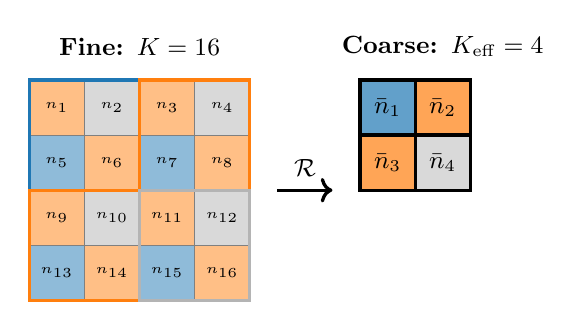
\begin{tikzpicture}[scale=0.70]
    % Fine grid 4x4
    \node[font=\small\bfseries] at (2,4.6) {Fine: $K=16$};
    \foreach \i in {0,...,3} \foreach \j in {0,...,3} {
      \pgfmathsetmacro\col{mod(\i/2,1)<0.5 ? (mod(\j/2,1)<0.5 ? "settledblue" : "activeorange") : (mod(\j/2,1)<0.5 ? "activeorange" : "emptygray")}
      \fill[\col,opacity=0.5] (\j,\i) rectangle (\j+1,\i+1);
      \draw[gray] (\j,\i) rectangle (\j+1,\i+1);
      \node[font=\tiny] at (\j+0.5,\i+0.5) {$n_{\pgfmathparse{int(4*(3-\i)+\j+1)}\pgfmathresult}$};
    }
    % Braces
    \draw[very thick,settledblue] (0,2) rectangle (2,4);
    \draw[very thick,activeorange] (2,2) rectangle (4,4);
    \draw[very thick,activeorange] (0,0) rectangle (2,2);
    \draw[very thick,emptygray] (2,0) rectangle (4,2);

    % Arrow
    \draw[->,very thick] (4.5,2) -- (5.5,2);
    \node[font=\small] at (5,2.4) {$\mathcal{R}$};

    % Coarse
    \node[font=\small\bfseries] at (7.5,4.6) {Coarse: $K_{\rm eff}=4$};
    \fill[settledblue,opacity=0.7] (6,3) rectangle (7,4);
    \fill[activeorange,opacity=0.7] (7,3) rectangle (8,4);
    \fill[activeorange,opacity=0.7] (6,2) rectangle (7,3);
    \fill[emptygray,opacity=0.5] (7,2) rectangle (8,3);
    \draw[very thick] (6,2) rectangle (8,4);
    \draw[very thick] (7,2) -- (7,4);
    \draw[very thick] (6,3) -- (8,3);
    \node[font=\small] at (6.5,3.5) {$\bar n_1$};
    \node[font=\small] at (7.5,3.5) {$\bar n_2$};
    \node[font=\small] at (6.5,2.5) {$\bar n_3$};
    \node[font=\small] at (7.5,2.5) {$\bar n_4$};
  \end{tikzpicture}
\end{column}
\end{columns}
\end{frame}

% ================================================================
%  6. The coarse RDME
% ================================================================
\begin{frame}{The coarse RDME: how rates change for merged patches}

For a patch $\mathcal{J}$ of $M_J$ voxels, the coarse state $\bar{n}_J$ evolves
under \textbf{patch-corrected} rates:

\bigskip
\begin{columns}[T]
\begin{column}{0.48\textwidth}
  \textbf{Reactions within patch $J$:}
  \begin{align*}
    \text{Birth: } &M_J \cdot \lambda \quad \text{(all voxels produce)}\\
    \text{Death: } &\mu\,\bar{n}_J \quad \text{(first-order, exact)}
  \end{align*}
  For nonlinear reactions (e.g.\ Schl\"{o}gl):
  rates use Multinomial moments within the patch.

  \bigskip
  \textbf{Diffusion between patches $J$ and $J'$:}
  \[
    \bar{n}_J \to \bar{n}_J - 1,\;\bar{n}_{J'} \to \bar{n}_{J'} + 1
  \]
  \[
    \text{rate} = \frac{D}{h^2}\cdot\frac{n_{\rm adj}(J,J')}{M_J}\cdot\bar{n}_J
  \]
  where $n_{\rm adj}(J,J')$ = shared boundary voxel pairs.
\end{column}
\begin{column}{0.48\textwidth}
  \centering
  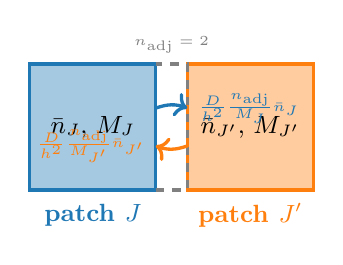
\begin{tikzpicture}[scale=0.8]
    % Patch J
    \fill[settledblue,opacity=0.4] (0,0) rectangle (2,2);
    \draw[settledblue,very thick] (0,0) rectangle (2,2);
    \node[font=\small] at (1,1) {$\bar{n}_J$, $M_J$};
    \node[settledblue,font=\small\bfseries] at (1,-0.4) {patch $J$};

    % Patch J'
    \fill[activeorange,opacity=0.4] (2.5,0) rectangle (4.5,2);
    \draw[activeorange,very thick] (2.5,0) rectangle (4.5,2);
    \node[font=\small] at (3.5,1) {$\bar{n}_{J'}$, $M_{J'}$};
    \node[activeorange,font=\small\bfseries] at (3.5,-0.4) {patch $J'$};

    % Boundary
    \draw[very thick,dashed,gray] (2,0) -- (2.5,0) -- (2.5,2) -- (2,2);
    \node[font=\tiny,gray] at (2.25,2.3) {$n_{\rm adj}=2$};

    % Arrows
    \draw[->,very thick,settledblue] (2.0,1.3) to[bend left=20] (2.5,1.3)
      node[right,font=\tiny,align=left] {$\frac{D}{h^2}\frac{n_{\rm adj}}{M_J}\bar{n}_J$};
    \draw[->,very thick,activeorange] (2.5,0.7) to[bend left=20] (2.0,0.7)
      node[left,font=\tiny,align=right] {$\frac{D}{h^2}\frac{n_{\rm adj}}{M_{J'}}\bar{n}_{J'}$};
  \end{tikzpicture}

  \medskip
  {\small \textbf{Boundary-molecule approximation:}\\
   Each molecule is equally likely to be\\
   in any of the $M_J$ voxels.\\
   Exact in the fast-diffusion limit.}
\end{column}
\end{columns}
\end{frame}

% ================================================================
%  7. Prolongation: Multinomial splitting
% ================================================================
\begin{frame}{Prolongation: reconstructing fine marginals from coarse}

\begin{columns}[T]
\begin{column}{0.52\textwidth}
  The \textbf{prolongation} $\mathcal{P}$ reconstructs the fine-voxel
  distribution from the coarse marginal.

  \bigskip
  For a patch $\mathcal{J}$ of $M$ voxels with total $\bar{n}_J$:
  \[
    (n_{k_1},\ldots,n_{k_M}) \;\Big|\; \bar{n}_J
    \;\sim\; \Mult\!\left(\bar{n}_J;\;\tfrac{1}{M},\ldots,\tfrac{1}{M}\right)
  \]
  This is \textbf{exact} when within-patch diffusion is fast
  (diffusion equilibrium = Multinomial distribution).

  \bigskip
  Used for: plotting fine-grained means, coarsening decisions,
  and error estimates.

  \bigskip
  \begin{block}{For bistable reactions}
    The within-patch distribution is bimodal (not Multinomial).
    Use the quasi-stationary distribution (QSD) instead.
    \citeref{Dendukuri \& Khammash, in prep.}
  \end{block}
\end{column}
\begin{column}{0.45\textwidth}
  \centering
  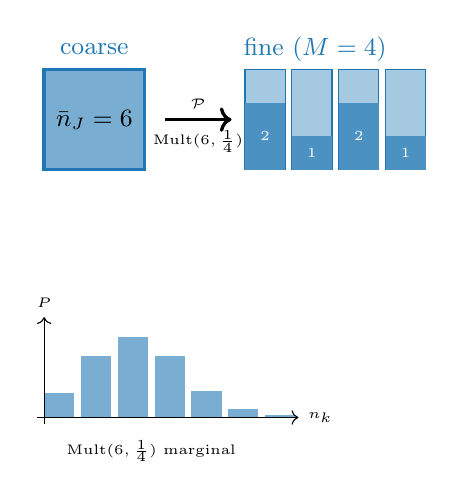
\begin{tikzpicture}[scale=0.85]
    % Coarse
    \fill[settledblue,opacity=0.6] (0,2.5) rectangle (1.5,4);
    \draw[settledblue,very thick] (0,2.5) rectangle (1.5,4);
    \node[font=\small\bfseries] at (0.75,3.25) {$\bar{n}_J = 6$};
    \node[font=\small,settledblue] at (0.75,4.3) {coarse};

    % Arrow
    \draw[->,very thick] (1.8,3.25) -- (2.8,3.25)
      node[midway,above,font=\tiny] {$\mathcal{P}$}
      node[midway,below,font=\tiny] {Mult$(6,\tfrac{1}{4})$};

    % Fine: 4 voxels
    \foreach \j/\n in {0/2, 1/1, 2/2, 3/1} {
      \fill[settledblue,opacity=0.4] (\j*0.7+3, 2.5) rectangle (\j*0.7+3.6,4);
      \draw[settledblue] (\j*0.7+3, 2.5) rectangle (\j*0.7+3.6,4);
      \fill[white] (\j*0.7+3,2.5) rectangle (\j*0.7+3.6, 2.5+\n*0.5);
      \fill[settledblue,opacity=0.8] (\j*0.7+3,2.5) rectangle (\j*0.7+3.6, 2.5+\n*0.5);
      \node[font=\tiny,white] at (\j*0.7+3.3, 2.5+\n*0.25) {\n};
    }
    \node[font=\small,settledblue] at (4.05,4.3) {fine ($M=4$)};

    % Distribution plot
    \begin{scope}[yshift=-1.2cm]
      \foreach \n/\p in {0/0.09, 1/0.23, 2/0.30, 3/0.23, 4/0.10, 5/0.03, 6/0.01} {
        \fill[settledblue,opacity=0.6] (\n*0.55, 0) rectangle (\n*0.55+0.45, \p*4);
      }
      \draw[->] (-0.1,0) -- (3.8,0) node[right,font=\tiny] {$n_k$};
      \draw[->] (0,-0.1) -- (0,1.5) node[above,font=\tiny] {$P$};
      \node[font=\tiny] at (1.6,-0.5) {$\Mult(6,\tfrac{1}{4})$ marginal};
    \end{scope}
  \end{tikzpicture}
\end{column}
\end{columns}
\end{frame}

% ================================================================
%  8. The adaptive algorithm
% ================================================================
\begin{frame}{The adaptive 2D FSP algorithm}

\begin{columns}[T]
\begin{column}{0.50\textwidth}
  \textbf{At each time step:}
  \begin{enumerate}\setlength\itemsep{0.5em}
    \item \textbf{Solve} the coarse FSP for one time step:\\
          $p_{\mathcal{S}} \leftarrow e^{A_{\mathcal{S}}\Delta t}\,p_{\mathcal{S}}$
    \item \textbf{Prune} states with $p < \varepsilon$
    \item \textbf{Expand} FSP boundary by one shell
  \end{enumerate}

  \smallskip
  \textbf{Periodically (every $\tau$ steps):}
  \begin{enumerate}\setlength\itemsep{0.3em}\setcounter{enumi}{3}
    \item \textbf{Update} mean-field $\bar{n}_k(t)$ for each fine voxel
    \item \textbf{Reclassify} voxels: settled / active / empty
    \item \textbf{Find} connected components $\to$ new CoarseningMap
    \item \textbf{If $K_{\rm eff}$ changed}: rebuild coarse system
  \end{enumerate}

  \medskip
  \textbf{Output:} prolong coarse marginals via Multinomial splitting.
\end{column}
\begin{column}{0.47\textwidth}
  \centering
  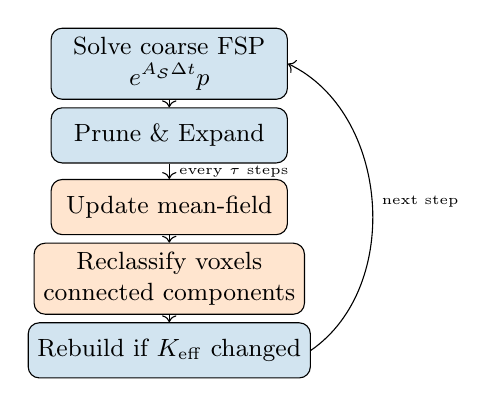
\begin{tikzpicture}[scale=0.7,
    box/.style={draw,rounded corners,minimum width=3.0cm,minimum height=0.7cm,
                font=\small,align=center}]
    \node[box,fill=myblue!20] (solve) at (0,5) {Solve coarse FSP\\$e^{A_{\mathcal{S}}\Delta t}p$};
    \node[box,fill=myblue!20] (prune) at (0,3.7) {Prune \& Expand};
    \node[box,fill=activeorange!20] (mf) at (0,2.4) {Update mean-field};
    \node[box,fill=activeorange!20] (coarsen) at (0,1.1) {Reclassify voxels\\connected components};
    \node[box,fill=settledblue!20] (rebuild) at (0,-0.2) {Rebuild if $K_{\rm eff}$ changed};

    \draw[->] (solve) -- (prune);
    \draw[->] (prune) -- (mf) node[midway,right,font=\tiny] {every $\tau$ steps};
    \draw[->] (mf) -- (coarsen);
    \draw[->] (coarsen) -- (rebuild);
    \draw[->] (rebuild.east) to[bend right=60] node[right,font=\tiny] {next step} (solve.east);
  \end{tikzpicture}
\end{column}
\end{columns}
\end{frame}

% ================================================================
%  9. 2D birth-death: the demo figure
% ================================================================
\begin{frame}{2D birth-death: adaptive coarsening tracks a radial wavefront}

\begin{center}
  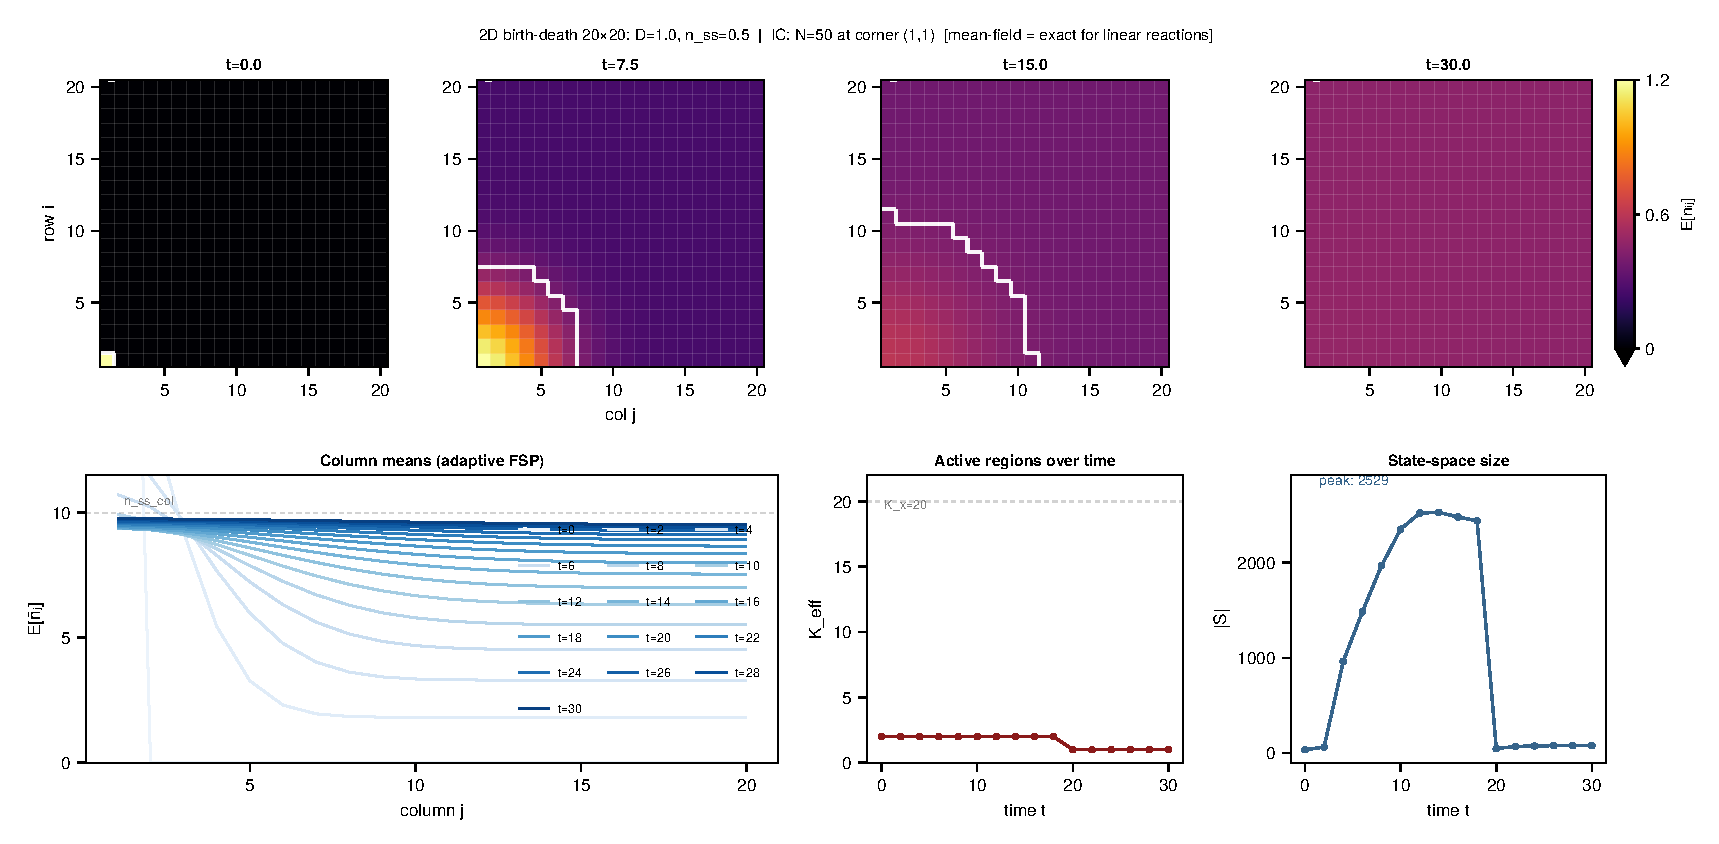
\includegraphics[width=0.92\textwidth]{fig_2d_birthdeath_adaptive}
\end{center}

\vspace{-0.3em}
{\small
  20$\times$20 grid, birth-death ($\lambda=0.05$, $\mu=0.1$, $n_{\rm ss}=0.5$),
  $D=1.0$, IC: $N=50$ molecules at corner $(1,1)$.\\[0.3em]
  \textbf{White lines}: coarse region boundaries.
  \textbf{Faint grid}: individual fine voxels.
  \textbf{K\_eff} annotated on each panel.
}
\end{frame}

% ================================================================
%  10. K_eff trajectory and state space
% ================================================================
\begin{frame}{$K_{\rm eff}$ grows and collapses to 1}

\begin{columns}[T]
\begin{column}{0.50\textwidth}
  \textbf{Algorithm behaviour:}
  \begin{itemize}\setlength\itemsep{0.5em}
    \item $t{=}0$: IC at corner $\to$ $K_{\rm eff}{=}2$
          (one settled + one empty)
    \item $t\in(0,19)$: wavefront spreads $\to$ $K_{\rm eff}{=}2$--$3$
          (settled corner / active front / empty bulk)
    \item $t{=}19$: all voxels reach $n_{\rm ss}$, spatial gradient
          vanishes $\to$ $K_{\rm eff}{=}1$
  \end{itemize}

  \bigskip
  \begin{alertblock}{$K_{\rm eff} = 1$ = pure CME}
    At $t{=}19$, the RDME collapses to a single
    super-voxel.  Only the \emph{total count} $N$ needs
    to be tracked.\\[0.3em]
    $|\mathcal{S}|$: 2529 $\to$ 78.
  \end{alertblock}
\end{column}
\begin{column}{0.47\textwidth}
  \textbf{Naive FSP vs adaptive:}

  \bigskip
  \begin{tabular}{lrr}
    \toprule
    & Naive FSP & Adaptive \\
    \midrule
    Dimensions & $K = 400$ & $K_{\rm eff} \le 3$ \\
    Max $|\mathcal{S}|$ & $n_{\max}^{400}$ & 2\,529 \\
    Wall time & $\infty$ & \textbf{2.3 s} \\
    \bottomrule
  \end{tabular}

  \bigskip
  \textbf{Complexity:} $|\mathcal{S}| \sim n_{\max}^{K_{\rm eff}}$\\
  The exponent tracks the wavefront,\\
  not the full grid.
\end{column}
\end{columns}
\end{frame}

% ================================================================
%  11. Why the staircase? 2D connected components
% ================================================================
\begin{frame}{The staircase boundary: 2D connected components}

\begin{columns}[T]
\begin{column}{0.50\textwidth}
  \textbf{Classification at $t = 7.5$:}\\[0.5em]
  Each fine voxel $(i,j)$ is labelled by its mean-field mean:
  \[
    \text{label} = \begin{cases}
      \text{settled} & \bar{n}_{ij} \ge \theta_{\rm hi}\\
      \text{active}  & \theta_{\rm lo} < \bar{n}_{ij} < \theta_{\rm hi}\\
      \text{empty}   & \bar{n}_{ij} \le \theta_{\rm lo}
    \end{cases}
  \]

  \smallskip
  Connected components of same-label voxels (4-connectivity)
  $\to$ each component is one super-voxel.

  \smallskip
  The \textbf{staircase} is the boundary between the
  settled/active component and the empty component.

  \medskip
  \begin{block}{Why connected components?}
    Within a connected same-label region, fast diffusion
    equilibrates molecules $\to$ distribution $\approx$ Multinomial
    $\to$ safe to merge.
  \end{block}
\end{column}
\begin{column}{0.47\textwidth}
  \centering
  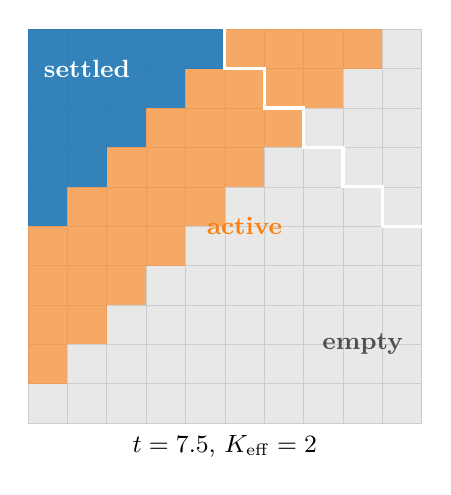
\begin{tikzpicture}[scale=0.5]
    % 10x10 grid at t=7.5 — settled (bottom-left), active (diagonal), empty (top-right)
    \foreach \i in {0,...,9} \foreach \j in {0,...,9} {
      \fill[emptygray,opacity=0.3] (\j,9-\i) rectangle (\j+1,10-\i);
      \draw[gray!40,very thin] (\j,9-\i) rectangle (\j+1,10-\i);
    }
    % settled: i+j < 5
    \foreach \i/\j in {0/0,0/1,0/2,0/3,0/4,1/0,1/1,1/2,1/3,2/0,2/1,2/2,3/0,3/1,4/0} {
      \fill[settledblue,opacity=0.9] (\j,9-\i) rectangle (\j+1,10-\i);
    }
    % active: 5 <= i+j < 9
    \foreach \i/\j in {0/5,0/6,0/7,0/8,1/4,1/5,1/6,1/7,2/3,2/4,2/5,2/6,3/2,3/3,3/4,3/5,4/1,4/2,4/3,4/4,5/0,5/1,5/2,5/3,6/0,6/1,6/2,7/0,7/1,8/0} {
      \fill[activeorange,opacity=0.6] (\j,9-\i) rectangle (\j+1,10-\i);
    }
    % Staircase boundary
    \draw[white,very thick]
      (5,10)--(5,9)--(6,9)--(6,8)--(7,8)--(7,7)--(8,7)--(8,6)--(9,6)--(9,5)--(10,5);
    % Labels
    \node[white,font=\small\bfseries] at (1.5,9) {settled};
    \node[font=\small\bfseries,activeorange] at (5.5,5) {active};
    \node[font=\small\bfseries,mygray] at (8.5,2) {empty};
    \node[font=\small] at (5,-0.6) {$t=7.5$, $K_{\rm eff}=2$};
  \end{tikzpicture}
\end{column}
\end{columns}
\end{frame}

% ================================================================
%  12. Extension: Schlögl bistable wavefront
% ================================================================
\begin{frame}{Extension: bistable reactions (Schl\"{o}gl model)}

\begin{columns}[T]
\begin{column}{0.52\textwidth}
  \textbf{Schl\"{o}gl model:} bistable kinetics with two stable
  fixed points $n_{\rm lo}$ and $n_{\rm hi}$.

  \medskip
  Each voxel is in one of two phases.
  A sharp wavefront separates the phases and propagates across the grid.

  \bigskip
  \textbf{Challenges vs linear case:}
  \begin{itemize}\setlength\itemsep{0.4em}
    \item Within-patch distribution is \emph{bimodal}, not Multinomial
    \item Prolongation uses the \textbf{quasi-stationary distribution} (QSD)
          instead of Multinomial splitting
    \item Coarse reaction rates are non-trivial (Binomial moments)
  \end{itemize}

  \bigskip
  \textbf{Same coarsening structure:}\\
  $n_{\rm lo}$ voxels $\to$ merged, $n_{\rm hi}$ voxels $\to$ merged,
  transition voxels $\to$ fine.
\end{column}
\begin{column}{0.45\textwidth}
  \centering
  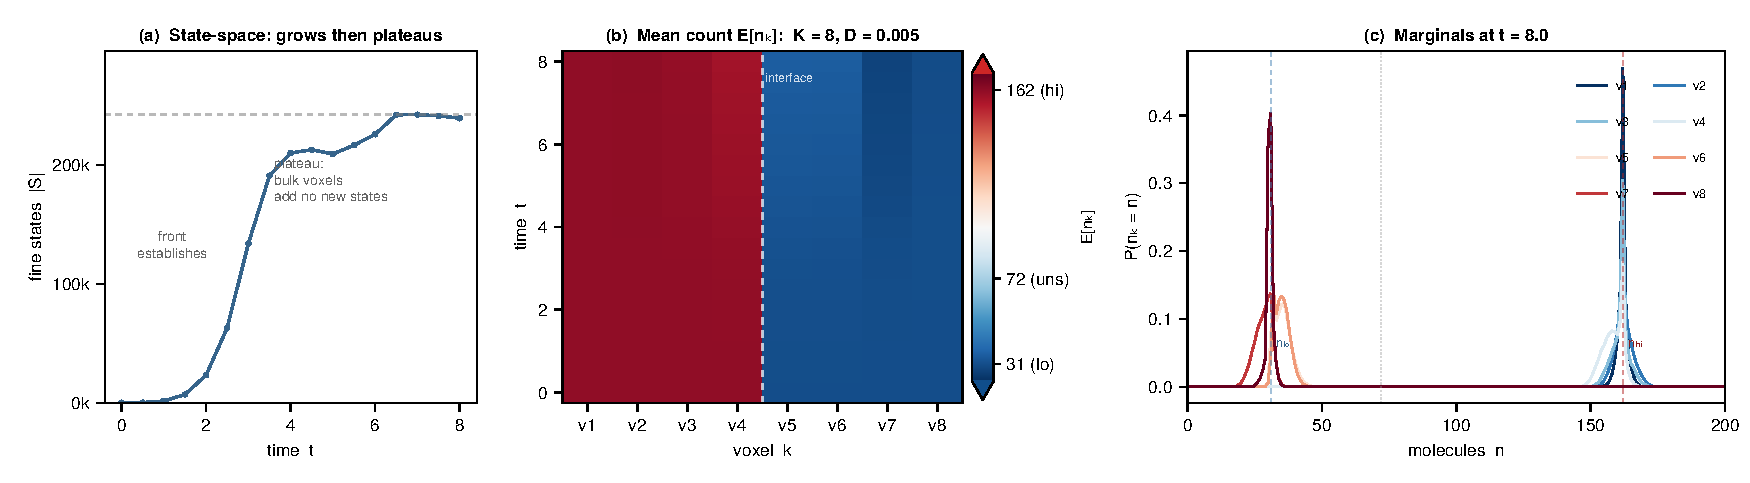
\includegraphics[width=\textwidth]{fig_k8_front}\\[0.5em]
  {\small K=8 Schl\"{o}gl wavefront via adaptive coarsening}
\end{column}
\end{columns}
\end{frame}

% ================================================================
%  13. Complexity and state space reduction
% ================================================================
\begin{frame}{State space complexity: the role of $K_{\rm eff}$}

\begin{columns}[T]
\begin{column}{0.55\textwidth}
  \textbf{Naive RDME FSP:} $|\mathcal{S}| \sim n_{\max}^K$ \\
  Exponential in the number of voxels.

  \bigskip
  \textbf{Adaptive coarse FSP:} $|\mathcal{S}| \sim n_{\max}^{K_{\rm eff}}$ \\
  Exponential only in the number of \emph{active} regions.

  \bigskip
  \begin{block}{$K_{\rm eff}$ is bounded by the wavefront}
    At any time, the number of dynamically distinct
    regions is small:
    \[
      K_{\rm eff} \le N_{\rm settled} + N_{\rm front} + N_{\rm empty}
    \]
    For a 2D wavefront: $K_{\rm eff} \approx 2$--$5$ even as $K \to \infty$.
  \end{block}

  \medskip
  \textbf{Limiting cases:} $K_{\rm eff}{=}K$ (full RDME) \;$\leftrightarrow$\; $K_{\rm eff}{=}1$ (CME)
\end{column}
\begin{column}{0.42\textwidth}
  \centering
  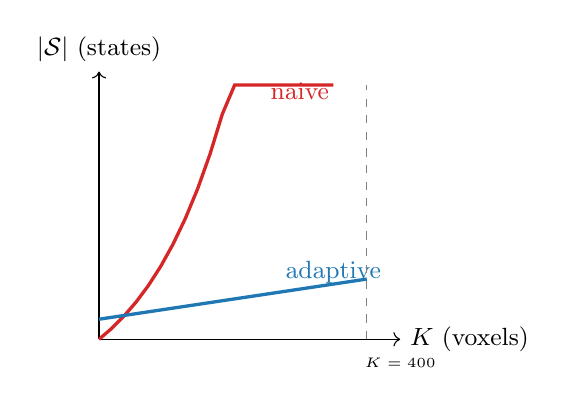
\begin{tikzpicture}[scale=0.85]
    \draw[->] (0,0) -- (4.5,0) node[right,font=\small] {$K$ (voxels)};
    \draw[->] (0,0) -- (0,4) node[above,font=\small] {$|\mathcal{S}|$ (states)};

    % Naive: exponential
    \draw[very thick,slowred] plot[domain=0:3.5,samples=20]
      (\x, {min(3.8, exp(\x*0.8)-1)});
    \node[slowred,font=\small] at (3.0,3.7) {naive};

    % Adaptive: nearly flat
    \draw[very thick,settledblue] plot[domain=0:4,samples=20]
      (\x, {0.3+0.15*\x});
    \node[settledblue,font=\small] at (3.5,1.0) {adaptive};

    \node[font=\tiny] at (4.5,-0.35) {$K=400$};
    \draw[dashed,gray] (4,0) -- (4,3.8);
  \end{tikzpicture}

  \medskip
  {\small For a propagating wavefront,\\
   $K_{\rm eff}$ stays bounded even as\\
   $K \to \infty$.}
\end{column}
\end{columns}
\end{frame}

% ================================================================
%  14. Implementation: the library
% ================================================================
\begin{frame}{Implementation: \texttt{DiscStochSim.jl}}

\begin{columns}[T]
\begin{column}{0.55\textwidth}
  \textbf{Key data structure: \texttt{CoarseningMap}}\\[0.4em]
  Encodes which fine voxels belong to each coarse region:
  \begin{itemize}
    \item \texttt{fine\_to\_coarse[k]}: coarse region for voxel $k$
    \item \texttt{coarse\_to\_fine[J]}: list of fine voxels in region $J$
  \end{itemize}

  \bigskip
  \textbf{Key functions:}
  \begin{itemize}\setlength\itemsep{0.4em}
    \item \texttt{build\_adaptive\_cmap\_2d}: connected-component\\
          coarsening from mean-field means
    \item \texttt{build\_rdme\_adaptive\_2d}: coarse RDME generator\\
          with correct 2D boundary-molecule diffusion
    \item \texttt{fine\_marginals\_from\_coarse}: Multinomial prolongation
    \item \texttt{build\_qsd\_table}: quasi-stationary distribution\\
          for bistable prolongation
  \end{itemize}

  \medskip
  {\small Works for any reaction network on any 2D grid.}
\end{column}
\begin{column}{0.42\textwidth}
  \centering
  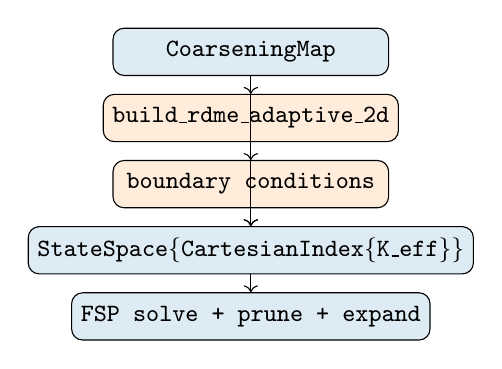
\begin{tikzpicture}[scale=0.7,
    box/.style={draw,rounded corners,minimum width=3.5cm,
                minimum height=0.6cm,font=\small\ttfamily,align=center}]

    \node[box,fill=settledblue!15] (cmap) at (0,4)
      {CoarseningMap};
    \node[box,fill=activeorange!15] (sys) at (0,2.8)
      {build\_rdme\_adaptive\_2d};
    \node[box,fill=activeorange!15] (bc) at (0,1.6)
      {boundary conditions};
    \node[box,fill=myblue!15] (sp) at (0,0.4)
      {StateSpace\{CartesianIndex\{K\_eff\}\}};
    \node[box,fill=myblue!15] (sol) at (0,-0.8)
      {FSP solve + prune + expand};

    \draw[->] (cmap) -- (sys);
    \draw[->] (cmap) -- (bc);
    \draw[->] (sys) -- (sp);
    \draw[->] (bc) -- (sp);
    \draw[->] (sp) -- (sol);
  \end{tikzpicture}
\end{column}
\end{columns}
\end{frame}

% ================================================================
%  15. Summary
% ================================================================
\begin{frame}{Summary}

\begin{columns}[T]
\begin{column}{0.55\textwidth}
  \textbf{Problem:} RDME state space grows as $n_{\max}^K$.\\
  Intractable for large spatial grids.

  \medskip
  \textbf{Insight:} voxels with low diffusion activity
  (settled or empty) can be safely merged.
  Only the active wavefront needs fine resolution.

  \medskip
  \textbf{Algorithm:}
  \begin{enumerate}\setlength\itemsep{0.3em}
    \item Classify voxels by mean-field mean
    \item Merge connected components into super-voxels
    \item Build coarse RDME with boundary-molecule diffusion
    \item Solve FSP on coarse state space
    \item Prolong to fine grid for output
  \end{enumerate}

  \medskip
  \textbf{Key result:} $K_{\rm eff} \ll K$ throughout;
  $K_{\rm eff} \to 1$ at SS (RDME $\to$ CME).
\end{column}
\begin{column}{0.42\textwidth}
  \centering
  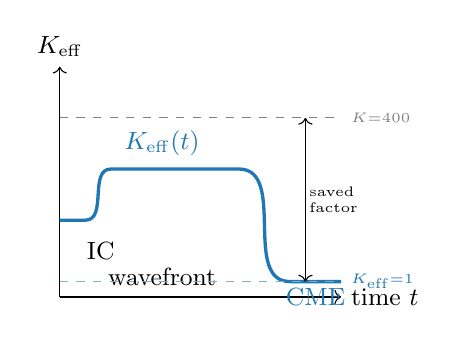
\begin{tikzpicture}[scale=0.65]
    % Axis
    \draw[->] (0,0) -- (5.5,0) node[right,font=\small] {time $t$};
    \draw[->] (0,0) -- (0,4.5) node[above,font=\small] {$K_{\rm eff}$};
    \draw[dashed,gray] (0,3.5) -- (5.5,3.5)
      node[right,font=\tiny,gray] {$K{=}400$};
    % K_eff curve: stays small, drops to 1
    \draw[very thick,settledblue]
      (0,1.5) -- (0.5,1.5) to[out=0,in=180] (1,2.5) -- (3.5,2.5)
      to[out=0,in=180] (4.5,0.3) -- (5.5,0.3);
    \node[settledblue,font=\small] at (2,3.0) {$K_{\rm eff}(t)$};
    \draw[<->] (4.8,0.3) -- (4.8,3.5);
    \node[font=\tiny,align=left] at (5.35,1.9)
      {saved\\factor};
    % Annotations
    \node[font=\tiny] at (0.8,0.9) {\small IC};
    \node[font=\tiny] at (2.0,0.4) {\small wavefront};
    \node[font=\tiny,settledblue] at (5.0,0.0) {\small CME};
    % K_eff = 1 line
    \draw[dashed,settledblue!60] (0,0.3) -- (5.5,0.3)
      node[right,font=\tiny,settledblue] {$K_{\rm eff}{=}1$};
  \end{tikzpicture}

  \bigskip
  \textbf{2D result:} 20$\times$20 grid, 6 seconds,\\
  $|\mathcal{S}|_{\max} = 2529$ vs $10^{400}$ (naive).
\end{column}
\end{columns}

\vspace{0.5em}
\begin{center}
  {\small Code: \texttt{DiscStochSim.jl} \quad $\bullet$ \quad
  Questions?}
\end{center}
\end{frame}

\end{document}
